\documentclass[11pt,letterpaper]{article}

\usepackage{fancyhdr}
\usepackage[latin1]{inputenc}
\usepackage{amsmath}
\usepackage{amsfonts}
\usepackage{amssymb}
\usepackage{graphicx}
\usepackage[hmargin=2cm,vmargin=2.5cm]{geometry}
\usepackage[normalem]{ulem}
\usepackage{enumerate}

\newcommand{\workingDate}{\textsc{7 January 2015}}
\newcommand{\courseName}{MTH 325 (Talbert)}
\newcommand{\institution}{Grand Valley State University}

\pagestyle{fancy}
\setlength\parindent{0in}
\setlength\parskip{0.1in}
\setlength\headheight{15pt}

%%%%%%%%%%% HEADER / FOOTER %%%%%%%%%%%
\rhead{\workingDate}
\chead{\textsc{Sample Work Activity}}
\lhead{\textsc{\courseName}}
\rfoot{\textsc{\thepage}}
\cfoot{\textit{Built: \today}}
\lfoot{\textsc{\institution}}

\begin{document}

As a part of working within our competency-based assessment system, we'll be spending time in class discussing what constitutes student work that receives a \textbf{Pass} mark and what constitutes a \textbf{No Pass} mark, so that you'll be able to judge your own work when the time comes, before handing it in. \\

In today's installment we have examples of student work (all made up by the professor, but realistic) that are solutions to the following problem: 
\begin{quote}
	Give an example of a function from $\mathbb{N}$ to $\mathbb{N}$ that is onto but not one-to-one. 
\end{quote}
Make the following assumptions about the context of the student work: 
\begin{itemize}
	\item This problem is part of a Learning Module but is not a proof. Therefore the work is subject to the ``Specifications for general writing'' and ``Specifications for mathematical problem solutions''. 
	\item Pretend that this is the ONLY item in the Learning Module. This is totally unrealistic, but we'll explain. 
	\item Each student below submitted their work on time and met all the technical formatting specifications. 
	\item Each student sample below is, verbatim, what the student submitted. 
\end{itemize}

As a reminder of the math: 
\begin{itemize}
	\item A function $f: A \rightarrow B$ is \emph{onto} if for every $b \in B$, there exists a point $a \in A$ such that $f(a) = b$. (Informally: Every point in the codomain is ``hit'' by at least one element in the domain.) 
	\item A function $f: A \rightarrow B$ is \emph{one-to-one} if, given $a_1, a_2 \in A$ with $a_1 \neq a_2$, we have $f(a_1) \neq f(a_2)$. (Informally: $f$ has ``no collisions'' where different points in the domain are sent to the same point in the codomain.) 
\end{itemize}

\subsection*{Student Sample 1} % (fold)
\label{sub:student_sample_1}

$f:\mathbb{N} \rightarrow \mathbb{N}$ given by $f(x) = \lfloor x \rfloor$. 

% subsection student_sample_1 (end)


\subsection*{Student Sample 2} % (fold)
\label{sub:student_sample_2}

The function $f:\mathbb{N} \rightarrow \mathbb{N}$ given by $f(x) = \lfloor x \rfloor$ is onto but not one-to-one because $f(2.1) = 2$ and $f(2.2) = 2$. 


% subsection student_sample_2 (end)

\subsection*{Student Sample 3} % (fold)
\label{sub:student_sample_3}

$f:\mathbb{N} \rightarrow \mathbb{N}$ given by $f(x) = \lfloor x \rfloor$ is onto but not one-to-one. $f$ is onto because, for example, if $5 \in \mathbb{N}$ then just plug in $5.1$ to the function and we get $f(5.1) = 5$, so every point in the codomain is hit by a point in the domain. The function is not one-to-one because $f(5.1) = 5$ and $f(5.2) = 5$. 

% subsection student_sample_3 (end)

\subsection*{Student Sample 4} % (fold)
\label{sub:student_sample_4}

The function $f:\mathbb{N} \rightarrow \mathbb{N}$ given by $f(x) = \lfloor x \rfloor$ is onto but not one-to-one. Here is a graph of this function: 
\begin{center}
	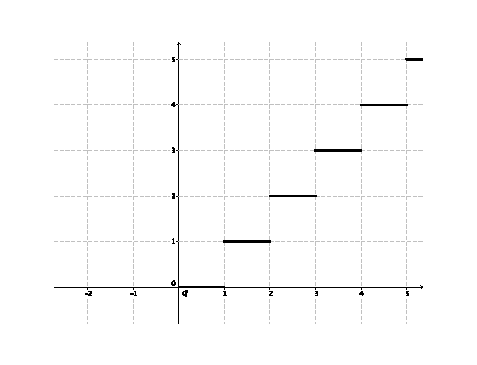
\includegraphics[width=0.3\textwidth]{sample1floor}
\end{center}
As we can see from the graph, the function passes the vertical line test and is therefore onto; and the function fails the horizontal line test and is therefore not one-to-one. 

% subsection student_sample_4 (end)


\subsection*{Student Sample 5} % (fold)
\label{sub:student_sample_5}

The function $g:\mathbb{N} \rightarrow \mathbb{N}$ given by $g(x) = x^2$ is onto but not one-to-one. The function $g$ satisfies the requirement that for every $b \in \mathbb{N}$ there exists $a \in \mathbb{N}$ such that $g(a) = b$, so $g$ is onto. However, we can see that $g(-2) = 4$ and $g(2) = 4$ as well, so $g$ is not one-to-one. 


% subsection student_sample_5 (end)

\subsection*{Student Sample 6} % (fold)
\label{sub:student_sample_6}

The function $h:\mathbb{N} \rightarrow \mathbb{N}$ given by $f(x) = \lceil x \rceil$ is onto but not one-to-one. The function $h$ is onto because if $b$ is any natural number in the codomain, $h(b)$ maps onto $b$ since rounding down an integer doesn't change the integer. And $h$ is not one-to-one because $1.1$ and $1.2$ both map to the same integer ($2$). 


% subsection student_sample_6 (end)

\end{document}